\subsection{Convolution}

\begin{frame}[allowframebreaks]{Semantic Segmentation Idea: Convolution}
\begin{figure}
\centering
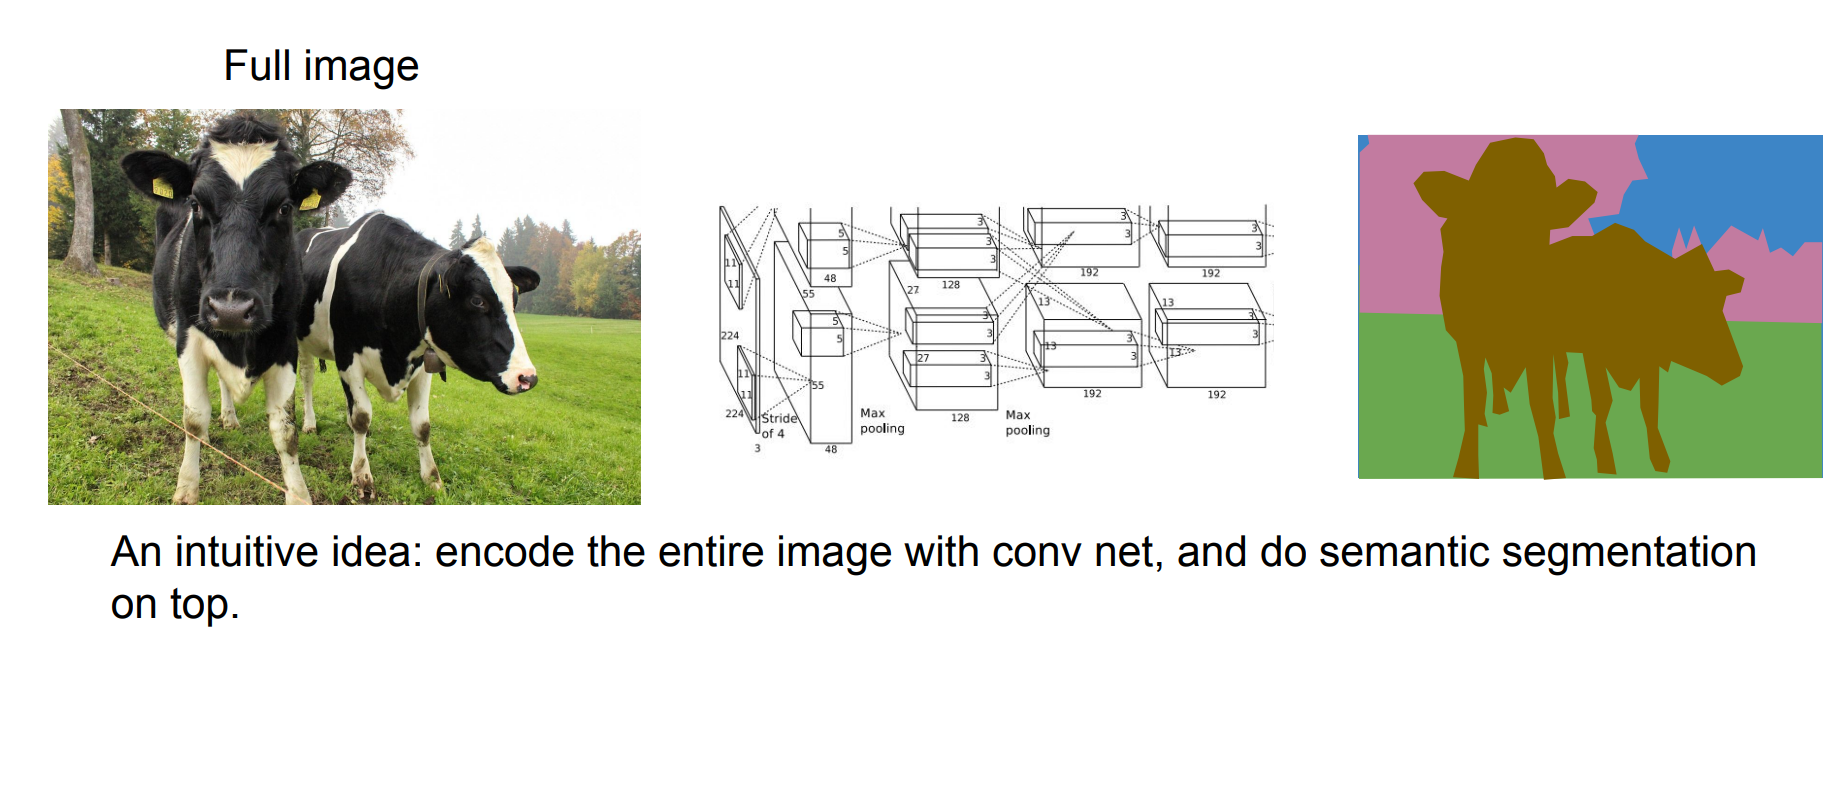
\includegraphics[width=1.0\textwidth,height=0.80\textheight,keepaspectratio]{images/segmentation/sem_5.png}
\caption*{\tiny Source: Stanford CS231n (2022), Lecture 9: Object Detection and Image Segmentation, slide 11}
\end{figure}

\framebreak

\begin{figure}
\centering
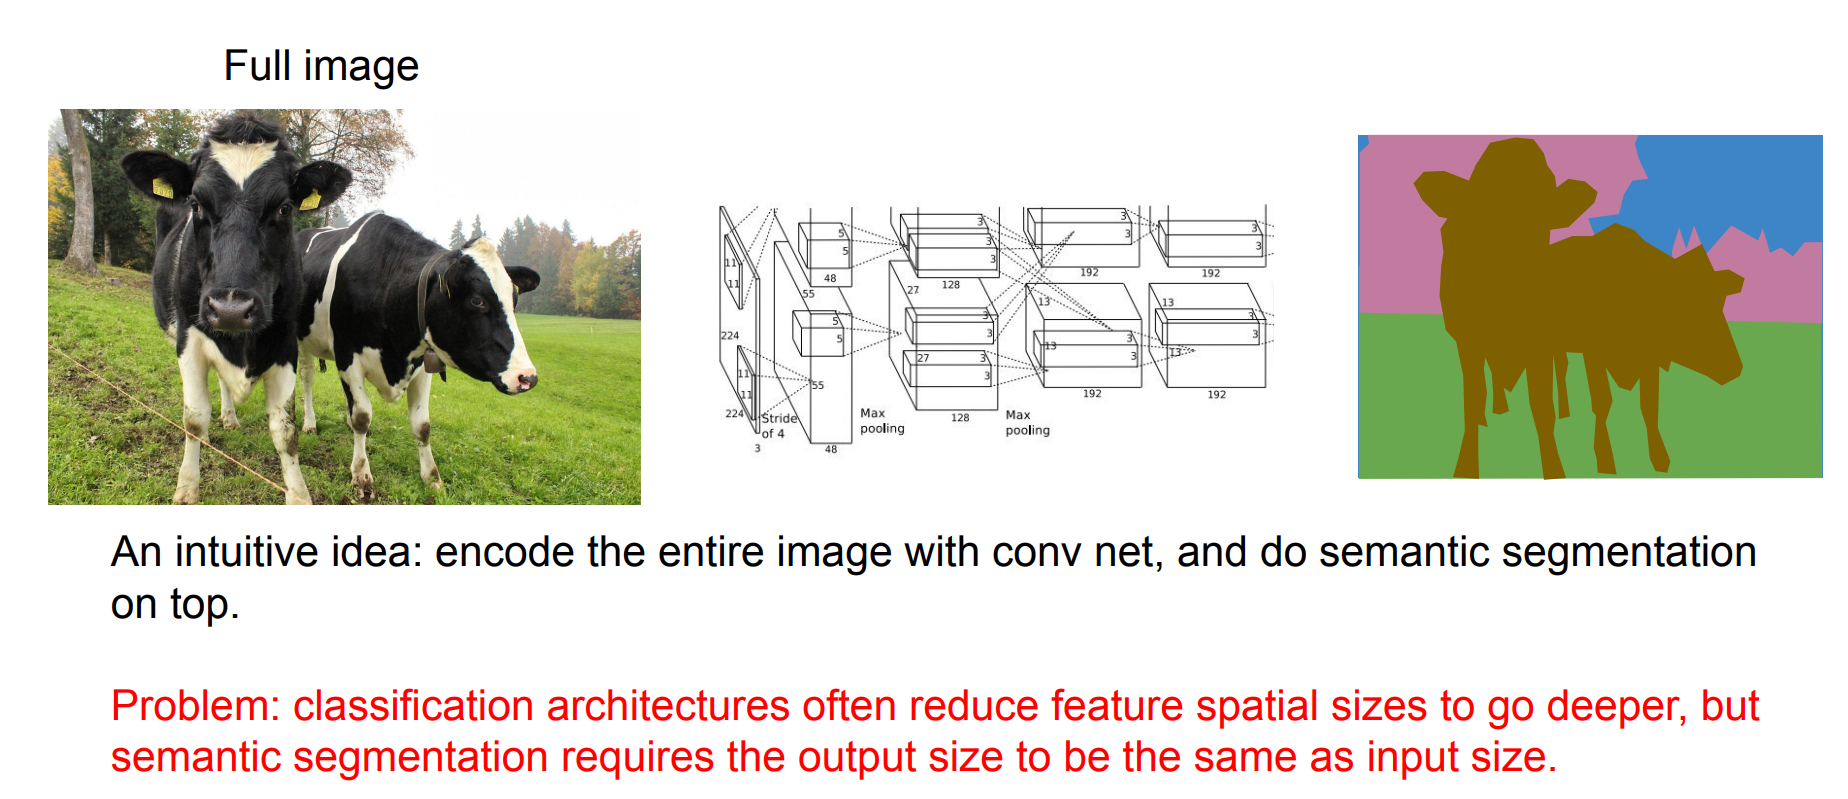
\includegraphics[width=1.0\textwidth,height=0.80\textheight,keepaspectratio]{images/segmentation/sem_6.png}
\caption*{\tiny Source: Stanford CS231n (2022), Lecture 9: Object Detection and Image Segmentation, slide 11}
\end{figure}
\end{frame}

\begin{frame}[allowframebreaks]{Semantic Segmentation Idea: Fully Convolutional}
\begin{figure}
\centering
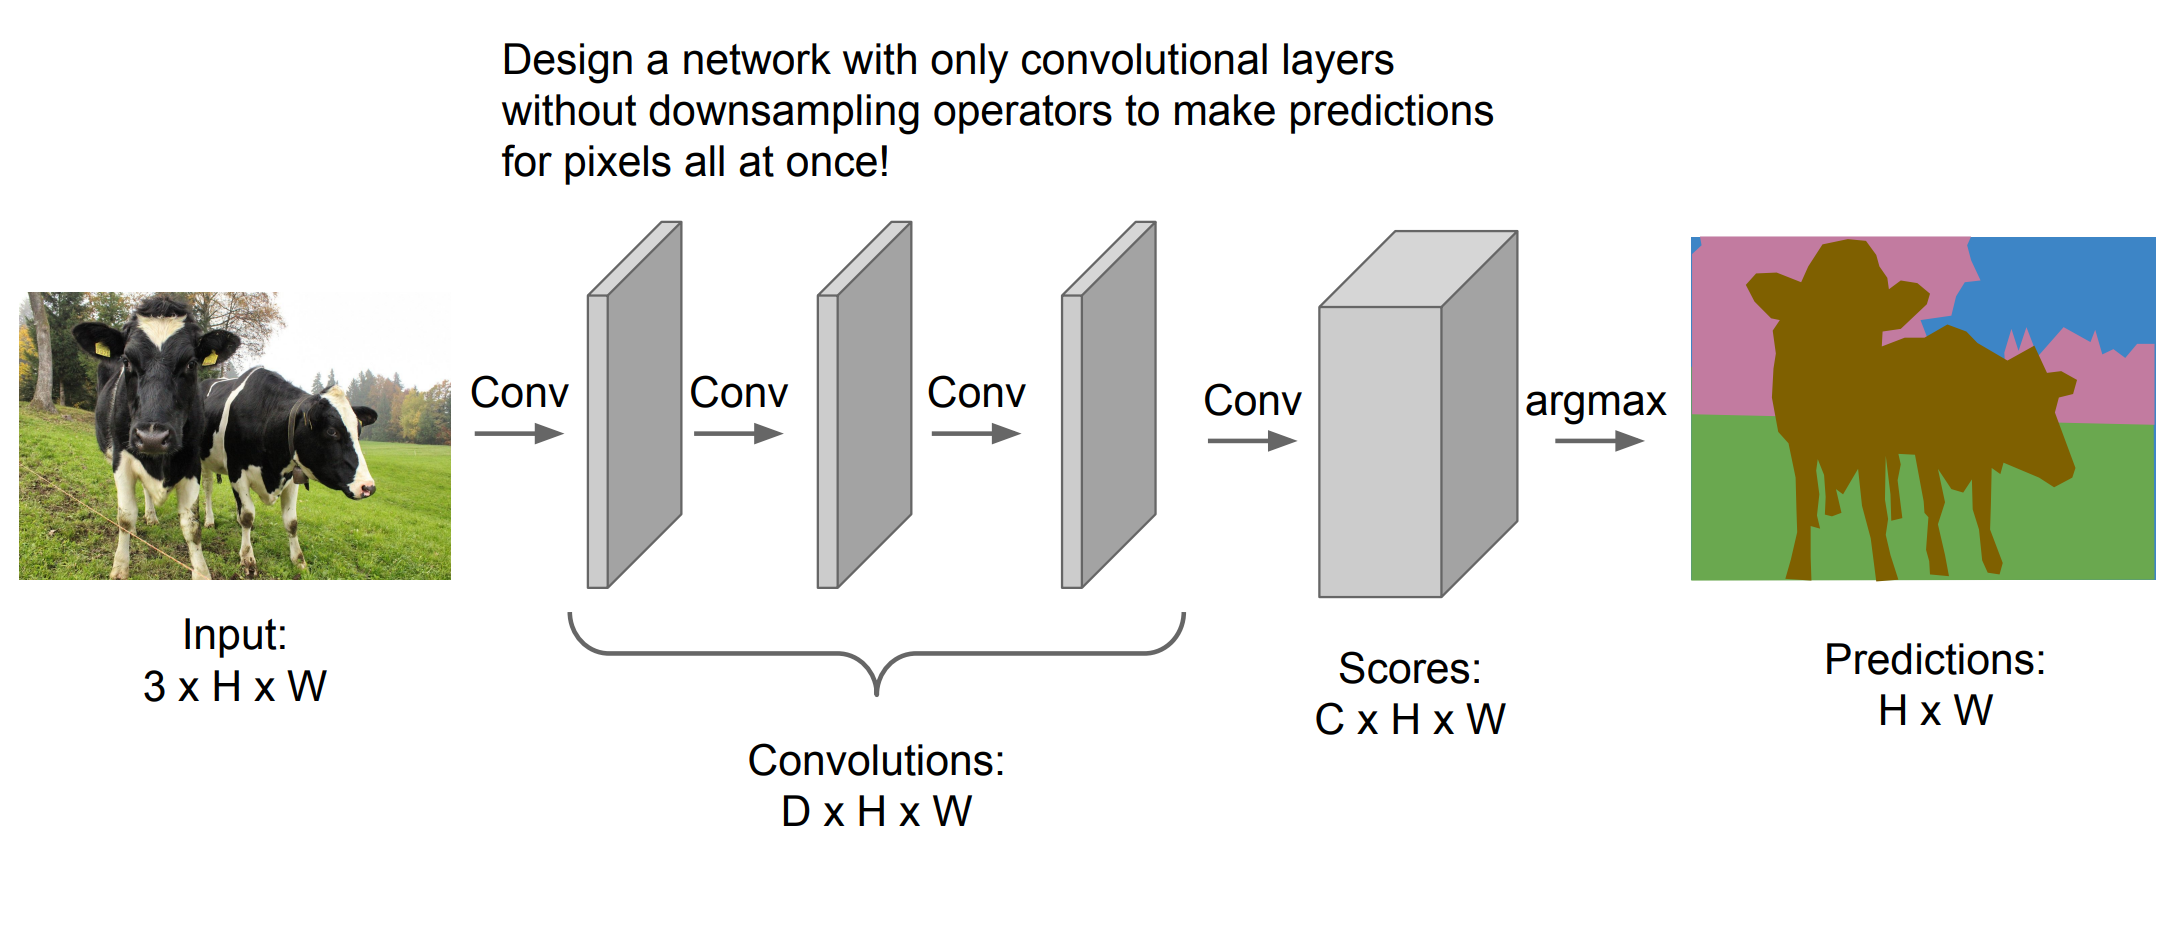
\includegraphics[width=1.0\textwidth,height=0.85\textheight,keepaspectratio]{images/segmentation/sem_7.png}
\caption*{\tiny Source: Stanford CS231n (2022), Lecture 9: Object Detection and Image Segmentation, slide 12}
\end{figure}

\framebreak

\begin{figure}
\centering
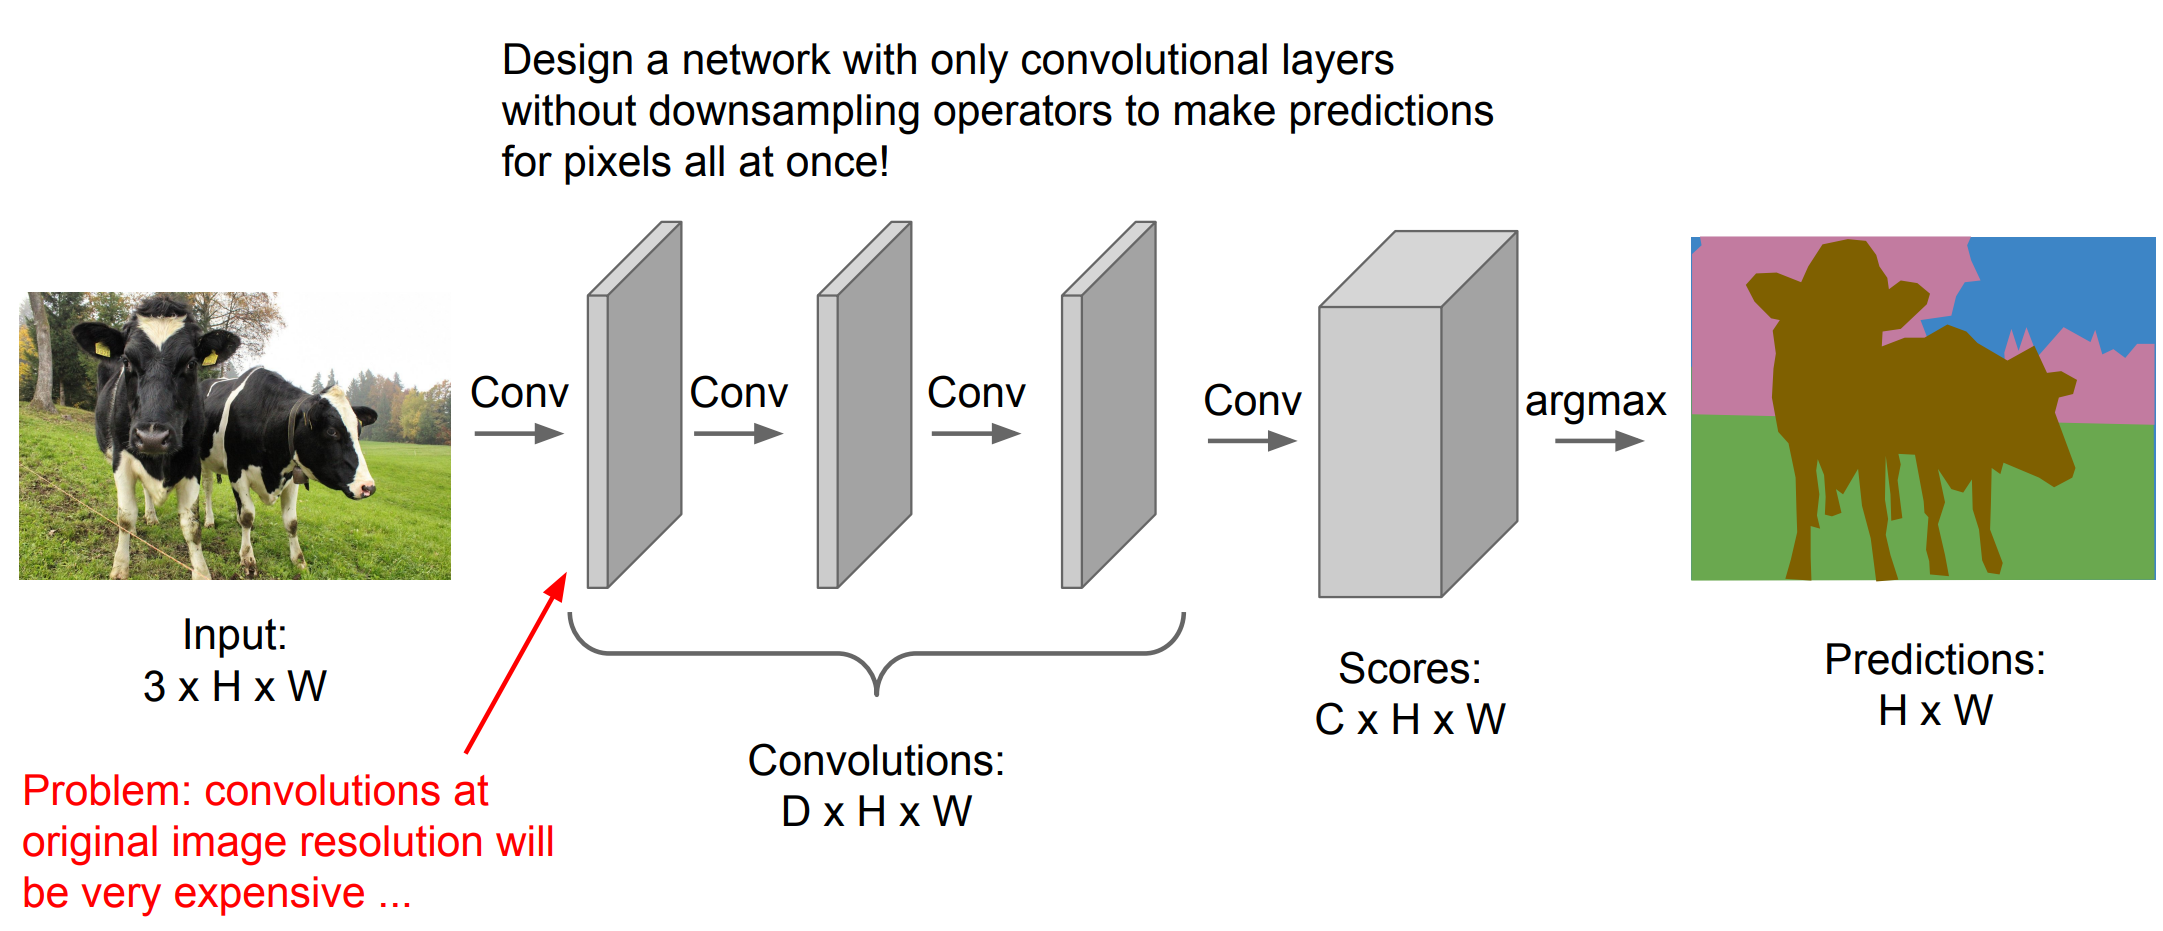
\includegraphics[width=1.0\textwidth,height=0.85\textheight,keepaspectratio]{images/segmentation/sem_8.png}
\caption*{\tiny Source: Stanford CS231n (2022), Lecture 9: Object Detection and Image Segmentation, slide 13}
\end{figure}

\framebreak

\begin{figure}
\centering
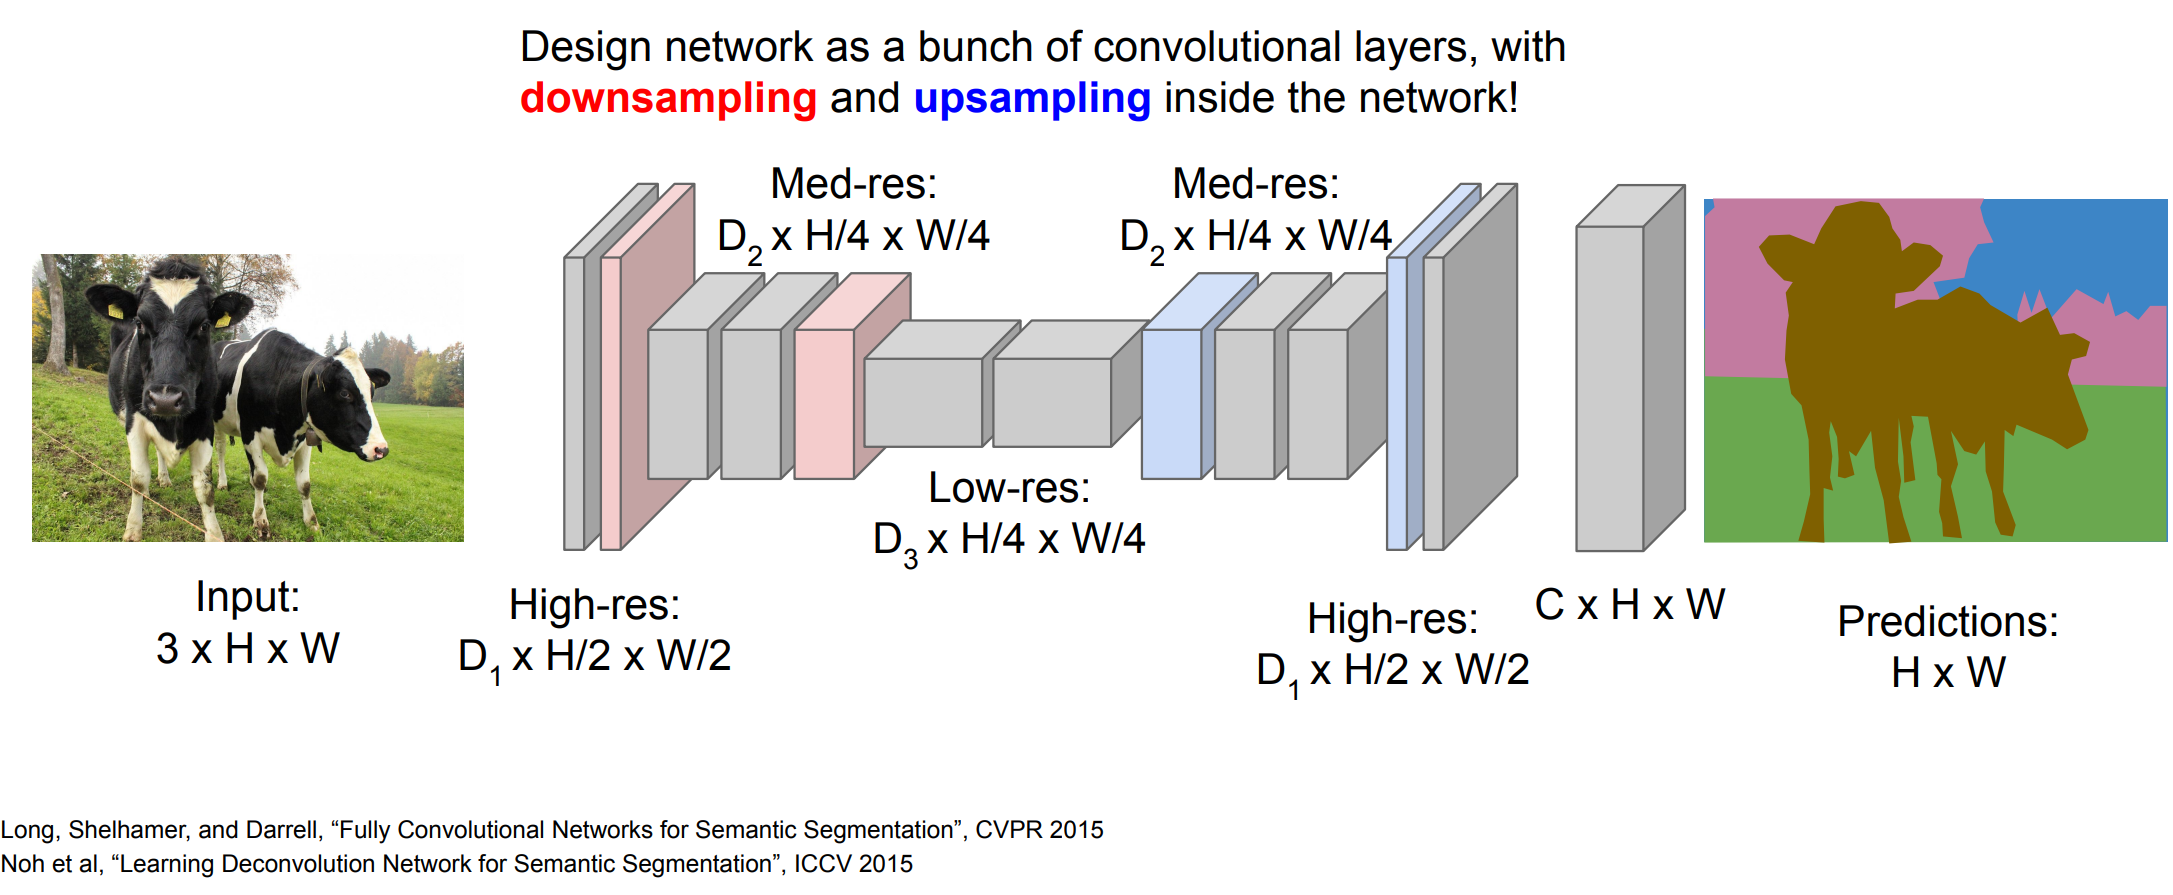
\includegraphics[width=1.0\textwidth,height=1.0\textheight,keepaspectratio]{images/segmentation/sem_9.png}
\end{figure}

\framebreak

\begin{figure}
\centering
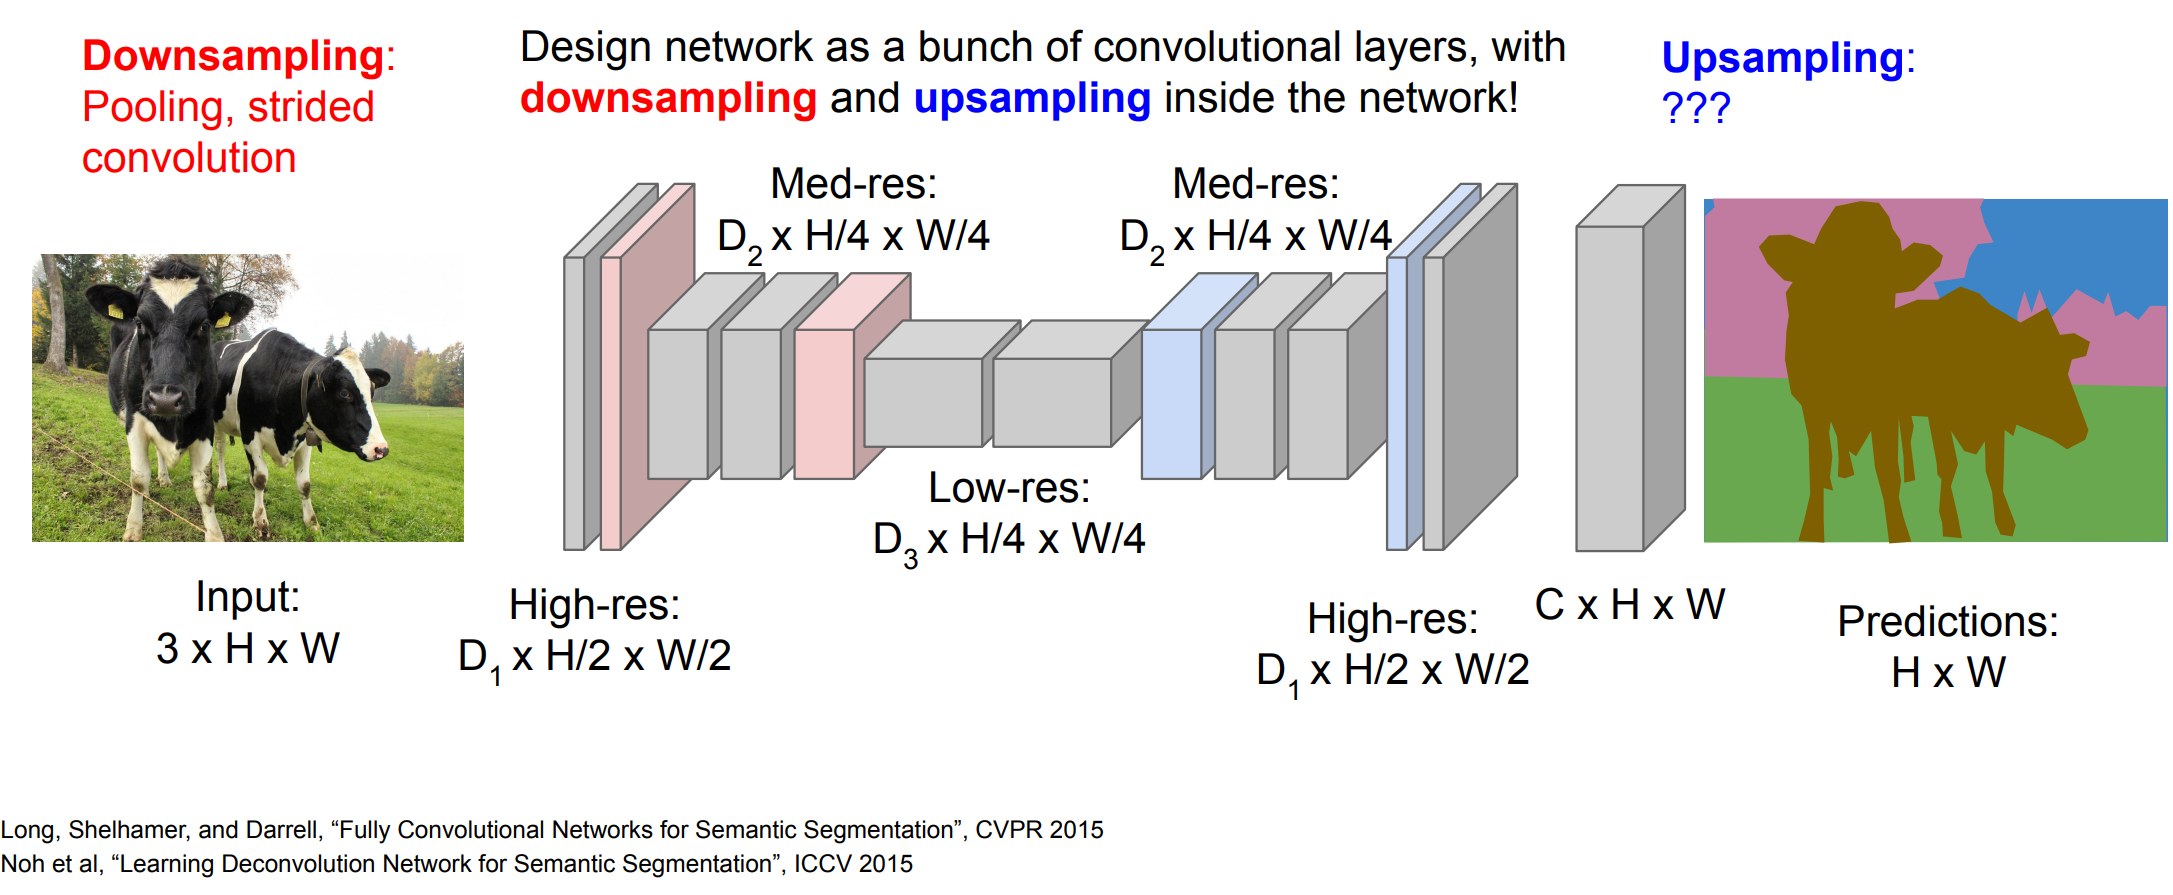
\includegraphics[width=1.0\textwidth,height=1.0\textheight,keepaspectratio]{images/segmentation/sem_10.png}
\end{figure}
    
\end{frame}

